\documentclass[tikz]{standalone}
\usetikzlibrary{arrows.meta}
\usepackage{mathtools}
\usepackage{amssymb}
\begin{document}
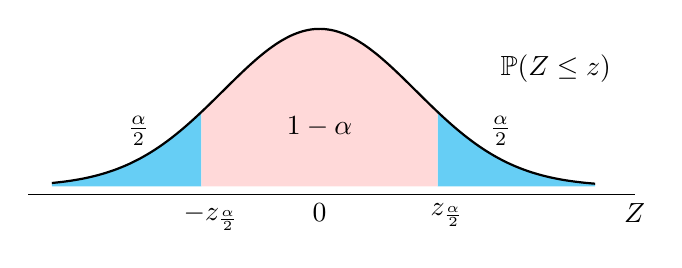
\begin{tikzpicture}[>={Stealth[length=6pt]},
  declare function={g(\x)=2*exp(-\x*\x/3);
    xmax=3.5;xmin=-3.4;x0=1.5;ymax=2.75;}]
 \draw[black] (-3.7,-0.1) edge[-] (4,-0.1);
 \fill[cyan!60] plot[domain=x0:xmax,samples=15,smooth] (\x,{g(\x)}) -- (xmax,0) -| cycle;  
 \fill[cyan!60] plot[domain=xmin:-1.5,samples=15,smooth] (\x,{g(\x)}) -- (-1.5,0) -| cycle;  
\fill[pink!60] plot[domain=-1.5:1.5,samples=15,smooth] (\x,{g(\x)}) -- (1.5,0) -- (-1.5,0) -- cycle;  
 \draw[thick] plot[domain=xmin:xmax,samples=51,smooth] (\x,{g(\x)}); 
 \path (0,-0.1) node[below]{0} (4,-0.1) node[below]{$Z$} (x0,-0.1) node[below]{\(z_{\mathrlap{\frac{\alpha}{2}}}\)} (-1.5,-0.1) node[below]{\(-z_{\mathrlap{\frac{\alpha}{2}}}\)} (-2.3, 0.4) node[above]{\(\frac{\alpha}{2}\)} (2.3, 0.4) node[above]{\(\frac{\alpha}{2}\)} (0, 0.5) node[above]{\(1 - \alpha\)} (3, 1.2) node[above]{\(\mathbb{P}(Z \leq z)\)};
\end{tikzpicture}
\end{document}